\skriptsection{Filtering in the Spatial Domain (V3)}{144}

\begin{tabular}{ll}
\parbox{7.5cm}{
  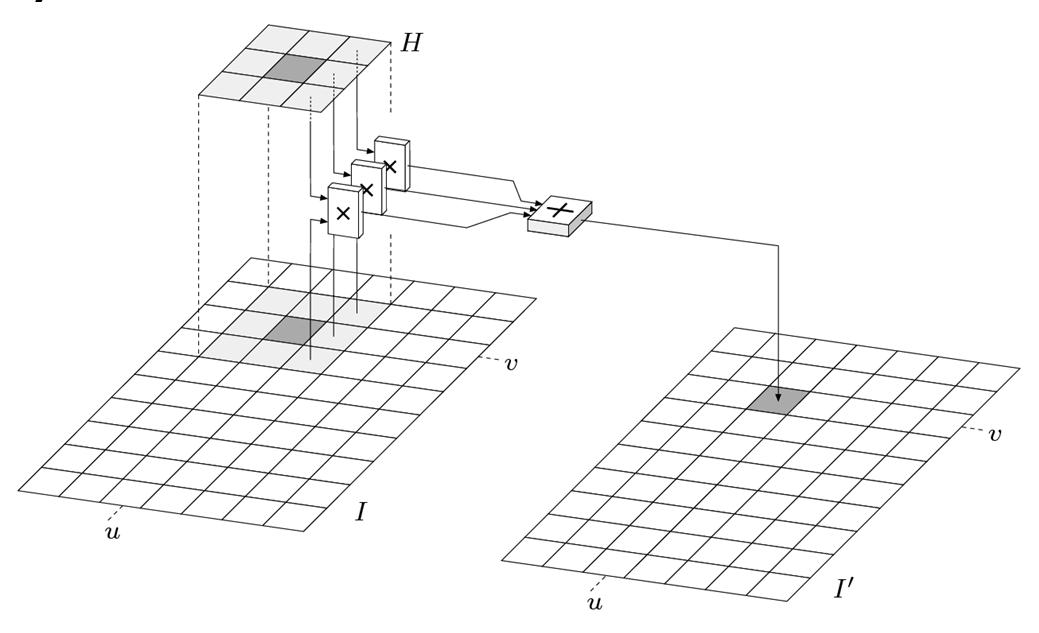
\includegraphics[width=7cm]{./images/filter_matrix.png}}
& \parbox{10cm}{
  Operations on images working with the pixels in the neighbourhood. This is a convolution of image 
  and filter matrix in the spatial domain.
  $$I' = I \ast H$$
  If H is 3x3 matrix and the origin is the center position:
  $$I' = \sum_{i=-1}^{1} \sum_{j=-1}^{1} I(u+i, v+j) \cdot H(i,j)$$
  
  Beware, to reach an image with the same intensity levels, the calculation should be 
  normalized either by dividing every pixel by the sum of the structural element (SE, $H$) or
  by normalizing the SE ($\sum_j \sum_k H_{jk} = 1$). 
}
\end{tabular}

\subsection{Filter Types}
  \label{sec:filter_types}
\begin{liste}
  \item Box lowpass filter (linear): $H_{3x3}= \begin{bmatrix}
   1 & 1 & 1\\
   1 & 1 & 1\\
   1 & 1 & 1\\
  \end{bmatrix}$
  
  \item Gaussian lowpass filter (linear): 
  $H_{3x3}= \begin{bmatrix}
   1 & 2 & 1\\
   2 & 4 & 2\\
   1 & 2 & 1 \\
  \end{bmatrix}$
  $H_{5x5} = \begin{bmatrix}
   0 & 1 & 2 & 1 & 0\\
   1 & 3 & 5 & 3 & 1\\
   2 & 5 & 9 & 5 & 2\\
   1 & 3 & 5 & 3 & 1\\
   0 & 1 & 2 & 1 & 0\\
  \end{bmatrix}$
  
  \item Rank filter (nonlinear): Select $k$th element of sorted neighbouring pixels
    \begin{liste}
      \item Median filter: Special form of a rank filter where the middle element is selected 
      (remove salt n' pepper noise): $\median(p_0, p_1, \ldots,p_k,\ldots,p_{2\cdot k}) = p_k$
      
      \item Minimum filter: Special form of a rank filter where the first element is selected 
      (eliminate white points, thickens dark regions)
      
      \item Maximum filter: Special form of a rank filter where the last element is selected 
      (eliminate dark points, thickens bright regions)
    \end{liste}
  
  \item Find edges in directions of zeros in structural element (gradient operators, based on first derivative)
  \begin{liste}
    \item Roberts $H_1^R = \begin{bmatrix}
      -1 & 0 \\ 0 & 1
    \end{bmatrix}$, $H_2^R = \begin{bmatrix}
      0 & -1\\ 1 & 0
    \end{bmatrix}$
    \item Prewitt
      $H_x^P =  \begin{bmatrix}
      -1 & 0 & 1\\
      -1 & 0 & 1\\
      -1 & 0 & 1\\
      \end{bmatrix}$
      $\quad 
      H_y^P =  \begin{bmatrix}
      -1 & -1 & -1\\
      0 & 0 & 0\\
      1 & 1 & 1\\
      \end{bmatrix}$
    \item Sobel (better noise suppression/smoothing than Prewitt):
      $H_x^S =  \begin{bmatrix}
      -1 & 0 & 1\\
      -2 & 0 & 2\\
      -1 & 0 & 1\\
      \end{bmatrix}$
      $\quad 
      H_y^S =  \begin{bmatrix}
      -1 & -2 & -1\\
      0 & 0 & 0\\
      1 & 2 & 1\\
      \end{bmatrix}$
    \item Compass edge filter (search edges in a specified direction, e.g. Kirsch):\\
      $H_0^K = H_x^S=  \begin{bmatrix}
      -1 & 0 & 1\\
      -2 & 0 & 2\\
      -1 & 0 & 1\\
      \end{bmatrix}$
      $\quad 
      H_1^K = \begin{bmatrix}
      -2 & -1 & 0\\
      -1 & 0 & 1\\
      0 & 1 & 2\\
      \end{bmatrix}$
      $\quad 
      H_2^K = H_y^S = \begin{bmatrix}
      -1 & -2 & -1\\
      0 & 0 & 0\\
      1 & 2 & 1\\
      \end{bmatrix}$
      $H_3^K = \begin{bmatrix}
      0 & -1 & -2\\
      1 & 0 & -1\\
      2 & 1 & 0\\
      \end{bmatrix}$
      $H_4^K = \begin{bmatrix}
      1 & 0 & -1\\
      2 & 0 & -2\\
      1 & 0 & -1\\
      \end{bmatrix}$
      $H_5^K = \begin{bmatrix}
      2 & 1 & 0\\
      1 & 0 & -1\\
      0 & -1 & -2\\
      \end{bmatrix}$
      $H_6^K = \begin{bmatrix}
      1 & 2 & 1\\
      0 & 0 & 0\\
      -1 & -2 & -1\\
      \end{bmatrix}$
      $H_7^K = \begin{bmatrix}
      0 & 1 & 2\\
      -1 & 0 & 1\\
      -2 & -1 & 0\\
      \end{bmatrix}$
  \end{liste}
  
  \item Laplacian (p. 160), edge intensities sharpening:  $\Lap(f(x,y)) = \frac{\delta^2f}{\delta x^2} + \frac{\delta^2f}{\delta y^2}$ 
    Beware of the \em double line effect \em which creates two lines per edge (one negative and one 
    positive due to the definition of the 2nd derivative. Elimination with zero-crossing detection).\\
    $H_{3 \times 3, anisotropic} = \begin{bmatrix}
     0 & -1 & 0\\
     -1 & 4 & -1\\
     0 & -1 & 0\\
    \end{bmatrix}$ \quad
      $H_{3 \times 3, isotropic} = \begin{bmatrix}
     -1 & -1 & -1\\
     -1 & 4 & -1\\
     -1 & -1 & -1\\
    \end{bmatrix}$ \quad
    $H_{5 \times 5, anisotropic} = \begin{bmatrix}
     0 & 0 & -1 & 0 & 0\\
     0 & -1 & -2 & -1 & 0\\
     -1 & -2 & 16 & -2 & -1\\
     0 & -1 & -2 & -1 & 0\\
     0 & 0 & -1 & 0 & 0\\
    \end{bmatrix}$
  
\end{liste}


\begin{minipage}{12cm}
  \subsection{Additional Comments}
    \subsubsection{Norm Smoothing Filters}
    All filter elements have to sum up to 1 in order to stay in the correct domain of intensity values.
    This is easily achievable by dividing all pixels by the sum of all filter elements.
    
    \subsubsection{Border Problems}
    It is not defined what happens at the borders. Therefore, computation is only possible at positions 
    completely inside picture. E.g. with a $3x3$ filter mask, the image border is $1$ and the resolution 
    is reduced by 2 in both directions (horizontally, vertically). Alternatively, the image can be 
    extended by constant values, by replicating pixels or by replicating cyclic.
\end{minipage}
\hspace{0.5cm}
\begin{minipage}{6.5cm}
\subsubsection{Derivatives}
  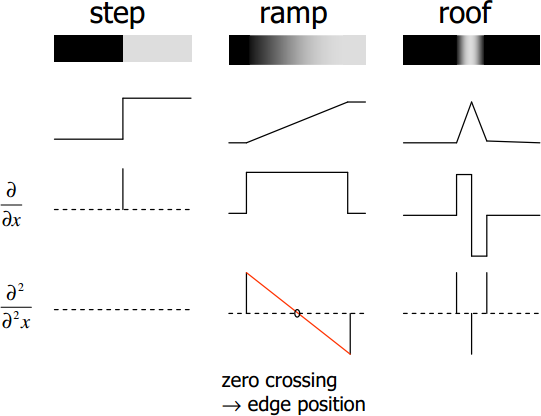
\includegraphics[width=5cm]{./images/derivatives.png}\\
  The second derivative is very sensible to noise (due to its highpass behaviour).
\end{minipage}
